% 
% Septiembre 2020
% Author: Mathieu Kessler
% Universidad Politécnica de Cartagena
% https://personas.upct.es/perfil/mathieu.kessler
% 
% 
\documentclass[handout,9pt]{beamer}
\definecolor{links}{HTML}{2A1B81}
\hypersetup{colorlinks,linkcolor=,urlcolor=links}
 \usepackage[spanish]{babel}
\usepackage{colortbl}
\usepackage{graphicx}
\usepackage{amsmath,amssymb}
\usepackage{comma}
\usepackage{fancybox,color}
\usepackage[utf8]{inputenc}
\graphicspath{{fig/}}
\setbeamertemplate{navigation symbols}{}
% -----------------------------------------------------------------------------
% To include multple images sequentially
% https://codeyarns.com/2010/02/09/how-to-do-image-animation-in-beamer/
% ------------------------------------------------------------------------------
 \usepackage{xmpmulti}
%------------------------------------------------------------------------------
\usepackage{xcolor}
\definecolor{mycodecolor}{rgb}{0.65,0.25,0.1}
\newcommand{\inlinecode}[1]{{\tt \textcolor{mycodecolor}{#1}}}
\usepackage{pythontex}
%--------------------
\usepackage{beamerthemeshadow}
\usepackage{xmpmulti}
\usepackage{mathtools}
\DeclarePairedDelimiter\abs{\lvert}{\rvert}%
\usepackage{tabularx}
\renewcommand\tabularxcolumn[1]{b{#1}}
\newcommand{\field}[1]{\mathbb{#1}}
\newcommand{\E}{\field{E}}
\newcommand{\R}{\field{R}}
\newcommand{\N}{\field{N}}
\newcommand{\Z}{\field{Z}}
\newcommand{\Q}{\field{Q}}
\newcommand{\EE}{\field{E}}
\newcommand{\FF}{\field{F}}
\newcommand{\GG}{\field{G}}
\renewcommand{\L}{\field{L}}
\renewcommand{\P}{\field{P}}
\newcommand{\LL}{{\mathfrak L}}

% define el folder donde del workspace, para cambiar inglés, ids,
% etc..
\newcommand{\workspacefolder}{stat\_labs }


\begin{document}
\title{Python: una introducción básica}

\author[Mathieu Kessler]{Mathieu Kessler}
\institute[]{Departamento de Matemática Aplicada y Estadística \\ Universidad Politécnica de Cartagena}
\date{@kessler\_mathieu}{}%{\href{https://code.visualstudio.com}{https://code.visualstudio.com}}
\titlegraphic{
\includegraphics[width=3cm]{../figures/python_logo}}

\begin{frame}
  \titlepage
\end{frame}

\begin{frame}
  \frametitle{Los principios básicos}
  \begin{enumerate}
  \item Los ficheros de programas Python tiene extensión \pyv{.py}
  \item Para introducir un comentario, usad  ``\#''
  \item Al ejecutar un fichero \inlinecode{.py} con
    \inlinecode{python myfile.py}, todas sus líneas son ejecutadas secuencialmente, desde la primera hasta la última.
  \item La indentación es una característica esencial de Python. Indica niveles jerarquizados de código.
  \item No es necesario declarar las variables como en C o Java etc...
  \item El tipo de datos de una variable es dinámico (es deducido de la primera aparición de la variable en el código)
  \item Se puede consultar el tipo de una variable \pyv{my_variable} con  \pyv{type(my_variable)}
  \end{enumerate}
\end{frame}
\begin{frame}[fragile]
  \frametitle{Las estructuras de datos básicas que vamos a usar}
  \begin{itemize}
    \item Entero (integer) \pyv{int}
    \item<2-> Flotante (Float) \pyv{float}\\\pause
      {\scriptsize
        \begin{minipage}{0.9\textwidth}
          \begin{block}{Qué es un número flotante?}
            "Float'' es una abreviatura para  "floating point." Es un tipo de datos fundamental presente en el compilador que se usa para definir valores numéricos con puntos decimales. Ej: 2.1562
          \end{block}
        \end{minipage}}
    \item<3-> Booleanos (Boolean)  \pyv{bool}\\ \pause
      {\scriptsize
        \begin{minipage}{0.9\textwidth}
          \begin{block}{Qué es un valor Booleano?}
            Una variable Booleana puede tomar dos valores:
            \pyv{True} o \pyv{False}. Se utiliza para expresar condiciones que permiten desencadenar acciones.
          \end{block}
        \end{minipage}}
    \item<4-> Cadenas (Strings) \pyv{str}
      {\scriptsize
        \begin{minipage}{0.9\textwidth}
          \begin{block}{Qué es una cadena?}
            \begin{itemize}\scriptsize
            \item Una cadena es una colección de caracteres. En Python, se enmarcan entre comillas simple, doble o triple: \pyv{'Hello!'}, \pyv{"Hello!"},
              \pyv{'''Hello!'''}.\\
            \item Puedes imprimir una cadena a la consola con \pyv{print}: 
              \pyv{print('Hello!')}\\
            \item Cadenas que abarquen múltiples líneas se pueden construir con comillas triples:
              \begin{pyblock}
print('''Esta cadena abarca 
                     varias líneas''')
              \end{pyblock}
            \end{itemize}
          \end{block}
        \end{minipage}}
  \end{itemize}
\end{frame}

\begin{frame}[fragile]
  \frametitle{Las estructuras de datos básicas que vamos a usar}
  \begin{itemize}
  \item Lista (list) \pyv{list}\\ \pause
    {\scriptsize
      \begin{minipage}{0.9\textwidth}
        \begin{block}{Qué es una lista en Python?}
         Una lista es una colección de elementos. Se escribe como una
         serie de valores separados por comas y enmarcados por corchetes\\
          Los elementos pueden tener tipos diferentes.\\
          Ejemplos: \\
          \pyv{mi_lista = [3.21, 4.87, -9.22]}\\
          \pyv{mi_lista = ['stats', 23, True]}\\
          En una lista, las posiciones de los elementos empiezan en 0,
          y para acceder a un elemento, se usan corchetes.
          \begin{pyconsole}
mi_lista = ['stats', 12, True]
print(mi_lista[0])
          \end{pyconsole}
        \end{block}
      \end{minipage}}\pause
  \item Tupla (Tuple) \pyv{tuple}\\ \pause
    {\scriptsize
      \begin{minipage}{0.9\textwidth}
        \begin{block}{Qué es un tuple en Python?}
          Un tuple es una colección de elementos. Se escribe como una
          serie de valores separados por comas y enmarcados entre paréntesis.\\
          Los elementos pueden tener tipos diferentes.\\
          Examples:\\
          \pyv{mi_tupla = (3.21, 4.87, -9.22)}\\
          \pyv{mi_tupla = ('stats', 23, True)}\\
          La diferencia con una lista es que un tupla es ``imutable'',
          lo que quiere decir que no se puede cambiar un elemento
          dentro de un tupla.\\
          Se accede a los elementos de un tupla de igual manera que
          para una lista.
        \end{block}
      \end{minipage}}
  \end{itemize}
\end{frame}

\begin{frame}[fragile]
  \frametitle{Las estructuras de datos básicas que vamos a usar}
  \begin{itemize}
  \item Conjunto (Set) \pyv{set}\\ \pause
    {\scriptsize
      \begin{minipage}{0.9\textwidth}
        \begin{block}{Qué es un conjunto en Python?}
          Un conjunto es una colección de elementos que no tiene
          ningún elemento duplicado. Se escribe como una serie de
          elementos separados por comas y enmarcados entre llaves.\\ 
          Los elementos pueden tener tipos diferentes. Se usan los
          conjuntos para llevar a cabo operaciones como unión,
          intersección, diferencia, etc. Ejemplos:\\ 
           \pyv{frutas = {'manzana',  'limón', 'banana'}}\\
               \pyv{verduras = {'tomate', 'zanahoria', 'berenjena'}}
        \end{block}
      \end{minipage}}\pause
  \item Diccionarios (Dictionaries) \pyv{dict}\\ \pause
    {\scriptsize
      \begin{minipage}{0.9\textwidth}
        \begin{block}{Qué es un diccionario en Python?}
          Un diccionario es una colección de elementos indexados. Sus
          elementos son de la forma clave:valor. Se pueden acceder a
          un elemento de un diccionario usándo su clave. Un diccionario se enmarca entre llaves.\\
          Sus elementos pueden ser de distintos tipos:
          Ejemplos:\\ \pyv{edades = {'john': 32,  'jane': 28, 'jim': 48}}\\
          Puede acceder al valor de un elemento indexando el
          diccionario por la clave del elemento entre corchetes:
          \begin{pyconsole}
edades = {'john': 32,  'jane': 28, 'jim': 48}
print(edades['jane'])
\end{pyconsole}
        \end{block}
      \end{minipage}}
  \end{itemize}
\end{frame}

\begin{frame}[fragile]
  \frametitle{Entrada y salida básica via la consola}
  \begin{itemize}
  \item \pyv{print} es la instrucción básica para imprimir objetos en
    la consola. \\
    Se puede imprimir cadenas:\\
    \begin{pyconsole}
print('Hello world!')
    \end{pyconsole}
    \pause
    pero también otros objetos directamente
    \begin{pyconsole}
edades = {'john': 32,  'jane': 28, 'jim': 48}
print(edades)
    \end{pyconsole}
  \item<3-> Para obtener valores o datos introducidos por el usuario
    en la consola, la instrucción es 
    \pyv{input}.
    \begin{pyverbatim}
>>> n = input('Número máximo de casos:')      
\end{pyverbatim}
\begin{pycode}
n = 4
\end{pycode}
\pause
Hay que tener en cuenta que la variable resultado del comando
\pyv{input} es de tipo cadena (str). Es posible que tenga que
transformarlo en entero o en float para su uso posterior:
\begin{pyverbatim}
>>> print(int(n) + 6)
\end{pyverbatim}
  \end{itemize}
\end{frame}
\begin{frame}[fragile]
  \frametitle{Bucles en Python}
  \begin{block}{El comando \pyv{for}}
    El comando \pyv{for} en Python permite iterar sobre los elementos
    de un objeto y ejecutar a cada iteración una series de instrucciones.
  \end{block}\pause
  \begin{itemize}
  \item Las instrucciones que se deben ejecutar en cada iteración
    están situadas en un bloque indentado debajo del comando \pyv{for}:\\
    \begin{pyverbatim}
for ciudad in ['Madrid', 'Murcia', 'Cartagena']:
    print(ciudad)
  \end{pyverbatim}
  \pause
 Otro ejemplo:\smallskip
 \begin{pyblock}
suma_final = 0
for i in (0, 1, 2, 3, 4, 5, 6):
    j = i * 2
    suma_final += j
print('El resultado final is: ' + str(suma_final))
\end{pyblock}
\pause
  \begin{block}{Notes}
    \begin{itemize}
    \item Para expresar la secuencia 0, 1, 2, 3, 4, 5, 6, podemos usar
      \pyv{range(6)}.    
      \item El operador \pyv{+=} indica el incremento propio, i.e
        \pyv{suma_final += j} es exactamente lo mismo que 
        \pyv{suma_final = suma_final + j}
      \item El operador \pyv{+} para dos cadenas lleva a cabo la
        concatenación. Para usarlo, hemos tenido que convertir primero
                \pyv{suma_final} en una cadena.
    \end{itemize}
  \end{block}
  \end{itemize}
\end{frame}
\begin{frame}[fragile]
  \frametitle{Ejercicios}
  \begin{enumerate}
    \item Escribe un programa en un fichero {\tt ejercicios\_introduccion.py} que
      pide un entero \pyv{n} al usuario y imprime en consola la suma
      de los primeros  \pyv{n} términos de la secuencia $4$, $-4/3$, $4/5$, $-4/7
      \ldots$, i.e. la secuencia
      $$ 4\times \frac{(-1)^{i}}{2\cdot i + 1},\ i = 0, 1, 2, \ldots$$
      \begin{itemize}
      \item \textit{Indicación 1: El operador de potencia en Python es
          \pyv{**}.}
      \item \textit{Indicación 2: Que no se os olvide de usar
          \pyv{int(n)} para transformar el input a un entero.}
      \end{itemize}
      Ejecutad vuestro programa con valores de $n$ grandes.
    \item Añadid a vuestro programa anterior
            las instrucciones para devolver la tabla de multiplicación
      de $n$, que ha introducido el usuario.
    \item Añadid a vuestro programa las instrucciones para imprimir el siguiente patrón:
      \begin{center}
        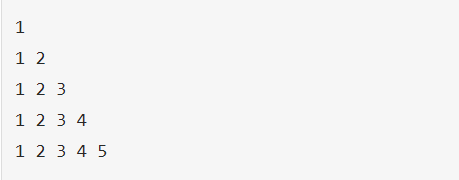
\includegraphics[width=5cm]{../figures/for_exercises_01}
      \end{center}
    \end{enumerate}  
  \end{frame}

\begin{frame}[fragile]
    \frametitle{Utilizar condiciones en nuestros programas}
    \begin{block}{Las instrucciones \pyv{if}, \pyv{if ... else},
        \pyv{if ... else ... elif}}
    La instrucción \pyv{if} en Python permite desencadenar acciones
    (instrucciones) si se cumple una condición
  \end{block}
  \pause
  \begin{itemize}
  \item   La estructura de la instrucción  \pyv{if} es similar al del
    bucle \pyv{for}, las instrucciones que deben ser ejecutadas si la
    condición se cumple se recojen en un bloque indentado debajo de la
    parte \pyv{if}
    {\scriptsize
    \begin{pyverbatim}
import math
n_string = input('Introduzca un número entero ')
n = int(n_string)
if (n > 0):
    print('La raiz cuadrada de  ' + str(n) + ' es ' + str(math.sqrt(n)))
  \end{pyverbatim}
}
\end{itemize}
\pause
\begin{block}{Note}
  La instrucción \pyv{import math} importa el módulo \pyv{math}, que
  contiene cientos de funciones matemáticas. Una vez el módulo
  importado, todas sus funciones están disponibles en nuestro
  programa. Para invocar una función de un  módulo,
  necesitamos añadirle el prefijo del módulo en el que está definido
  (en este caso \pyv{math}). Se verán más aspectos de los módulos más
  adelante.
\end{block}
\end{frame}
\begin{frame}
  \frametitle{Ejercicios}
  \begin{enumerate}
  \item Completad vuestro programa en {\tt ejercicios\_introduccion.py}
    con las  instrucciones para comprobar si $n$ introducido por el usuario es un
    número primo.
  \end{enumerate}  
\end{frame}

\begin{frame}[fragile]
  \frametitle{Funciones}
  \begin{overlayarea}{\textwidth}{\textheight}
  \begin{block}{}
    Las funciones permiten juntar una serie de instrucciones
    y llamarlas facilemente con un único comando (el nombre de la función)
  \end{block}
  \pause
  \begin{itemize}
  \item \pyv{def} es el comando que se usa para definir una función.
  \item Como siempre, la serie de instrucciones que deben ser
    ejecutadas cuando se invoca la función se situan en un bloque
    intentado debajo de \pyv{def}.a
  \item La función admite argumentos.
  \item La instrucción \pyv{return} se usa para devolver un valor
    (cualquier objeto de Python)
  \end{itemize}\pause
  Example:\vspace{-1cm}
  \begin{center}
    \multiinclude[format=png, graphics={width=7cm}]{../figures/function_example}
  \end{center}\pause\vspace{-0.5cm}
  
Una vez definida se puede invocar la función en un programa o en la consola:
\pyv{calculate_discount(121, 0.2)} devolverá el precio rebajado.\pause
  \begin{block}{Usad funciones!}
    El usar funciones es una práctica muy recomendable, mejora la
    legibilidad de vuestro código y su mantenimiento es más sencillo.
  \end{block}
\end{overlayarea}
\end{frame}

\begin{frame}[fragile]
  \frametitle{Funciones}
  \begin{block}{Recordad la función \pyv{calculate_discount}:}
    \begin{pyverbatim}
def calculate_discount(price, reduction):
    return price * (1 - reduction)
  \end{pyverbatim}
  \end{block}
  \begin{itemize}
  \item<2->   Cuando invocamos la función con  \pyv{calculate_discount(121, 0.2)},
  Python utiliza la posición de los valores proporcionados para
  asignarlos a los parámetros de la función
  the arguments.
  \begin{itemize}
  \item 121 está asignado al parámetro \pyv{price}
  \item 0.2 está asignado al parámetro \pyv{discount}
  \end{itemize}
\item<3-> Se pueden usar también los nombres de los
  parámetros cuando invocamos la función. En este caso su orden es irrelevante.
  \begin{pyverbatim}
calculate_discount(reduction=0.2, price=121) 
  \end{pyverbatim}
\item<4-> Debemos proporcionar el número correcto de valores cuando
  invocamos una función, excepto si se indicaron valores por defecto
  en la definición de la función:
  \begin{pyverbatim}
def calculate_discount(price, reduction=0.2):
    return price * (1 - reduction)
  \end{pyverbatim}
  En este caso, si se invoca la función con un único valor, éste se
  asignará al parámetro \pyv{price} y se aplicará un descuento de 20\%.
  \end{itemize}
\end{frame}

\begin{frame}[fragile]
  \frametitle{Funciones}
  \begin{block}{}
    Pensad en vosotros mismos y los posibles usuarios: documentad
    vuestro código!
  \end{block}\pause
  \begin{itemize}
  \item<2->   Python usa  Docstrings para proporcionar información
    sobre una función. Una docstring es una cadena que está situada
    como primera instrucción de una función (módulo, clase o método).
\item<3-> Dcstrings están enmarcadas por triples comillas:
 \pyv{"""Aquí viene el texto de información"""}
\item<4-> Para casos sencillos, se puede usar una docstring de una línea
  {\footnotesize
  \begin{pyverbatim}
def calculate_discount(price, reduction):
    """Devuelve el precio reducido"""
    return price * (1 - reduction)
  \end{pyverbatim}
  }
\item<5-> Usar docstrings permite al usuario obtener información vía
  \pyv{help}
  \begin{center}
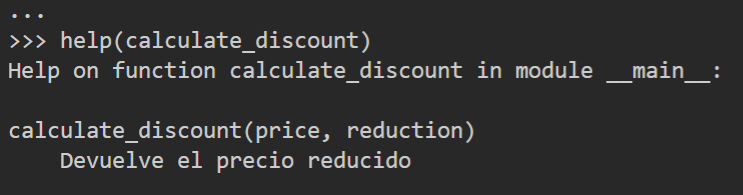
\includegraphics[width=8cm]{../figures/help_function_es}
\end{center}

\end{itemize}
\end{frame}

\begin{frame}[fragile]
  \frametitle{Ejercicios}
  \begin{enumerate}
  \item Añadid a vuestro programa en {\tt ejercicios\_introduccion.py}
    la definición de una función que tenga el entero \pyv{n} como
    argumento y que devuelva \pyv{True} si \pyv{n} es un número primo
    y  \pyv{False} en otro caso.
  \item Añadid al programa las instrucciones que permitan imprimir
    todos los números primos inferiores a \pyv{n}, introducido por el usuario.
  \end{enumerate}  
\end{frame}

\begin{frame}[fragile]
  \frametitle{Usando módulos}
  \begin{block}{Qué es un módulo?}
    Los módulos son ficheros con extensión {\tt .py} que contienen
    definiciones de funciones y objetos (variables, clases, etc...).
  \end{block}
  \begin{itemize}
  \item<2-> Si quiero usar las funciones de un módulo, debo
    importarlo. Por ejemplo, supongamos que he creado un fichero {\tt
      aux\_files.py} que contiene todas mis funciones útiles, lo
    importaré con 
    \begin{pyverbatim}
import aux_files
    \end{pyverbatim}
  \item<3-> Una vez que  \pyv{aux_file} está importado, si quiero
    invocar una de sus funciones, por ejemplo \pyv{calculate_discount} tendré que añadir como prefijo el
    nombre del módulo
    \begin{pyverbatim}
import aux_files
discounted_price = aux_files.calculate_discount(121, 0.2)      
    \end{pyverbatim}
  \item<4-> Para simplicar el código, puedo definir un alias para un
    módulo cuando lo importo:
        \begin{pyverbatim}
import aux_files as af
discounted_price = af.calculate_discount(121, 0.2)      
    \end{pyverbatim}
  \end{itemize}
\end{frame}

\begin{frame}[fragile]
  \frametitle{Usando módulos}
  \begin{itemize}
  \item<1-> Es posible importar sólo una o algunas funciones de un
    módulo determinado: 
    \begin{pyverbatim}
from aux_files import calculate_discount
    \end{pyverbatim}
  \item<2-> En este caso, no es necesario añadir el prefijo del módulo
    a la hora de invocar la función
    \begin{pyverbatim}
from aux_files import calculate_discount
discounted_price = calculate_discount(121, 0.2)      
    \end{pyverbatim}
  \item<3-> En algunos sitios podéis ver
        \begin{pyverbatim}
from aux_files import *
\end{pyverbatim}
Esto permitiría usar cualquier función del módulo \pyv{aux_files} sin
necesidad de añadir el prefijo del módulo. No es una buena práctica!
Es recomendado dejar constancia explícitamente de qué módulo proviene
la función que se usa.
  \end{itemize}
\end{frame}

\begin{frame}[fragile]
  \frametitle{Usando módulos}
  \begin{itemize}
  \item<1-> Python tiene una  \textit{ ``Librería estándar''
      (``Standard Library'')} de módulos útiles que vienen instalados
    con la distribución de Python. Además, existen miles de módulos
    compartidos por usuarios, preparados como \textit{``paquetes''
      (``packages'')} preparados para su descarga e instalación.
  \item<2-> Módulos de la  \textit{``Librería estándar} pueden ser
    importados directamente en mi código, usando  la instrucción
    \pyv{import}. Por ejemplo, el módulo  \pyv{math} mencionado anteriormente.
    \begin{pyverbatim}
import math
x = math.sin(0)
    \end{pyverbatim}
  \item<3-> Para usar módulos publicados por otros usuarios, es
    necesario descargar los paquetes asociados de los repositorios
    mantenidos por la comunidad.
  \item<4-> Uno de los repositorios muy importantes es  {\tt \tt PyPI}
    \href{https://pypi.org/}{https://pypi.org/}, the Python Package
    Index, un enorme repositorio de software desarrollado y compartido
    por la comunidad Python. Para descargar e instalar paquetes de
    {\tt PyPI}, se usa la utilidad  {\tt pip}. 
  \item<5-> Puesto que, en este curso, usamos la distribución
    Anaconda, no usaremos 
    {\tt pip} y {\tt PyPI}, sino la 
    \href{https://anaconda.org/}{Anaconda Cloud} y la instrucción  {\tt conda
      install}.
  \end{itemize}
\end{frame}

\begin{frame}[fragile]
  \frametitle{Usando módulos externos}
  \begin{itemize}
  \item Usaremos de manera intensa algunos de los módulos importantes
    para el cálculo científico, concretamente, {\tt numpy}, {\tt scipy},
    {\tt matplotlib} and {\tt pandas}.
  \item<2-> Si estás utilizando la distribución Anaconda completa,
    estos módulos ya están disponibles, basta con importarlos.
  \item<3-> Si estás utilizando la distribución  miniconda, tendrá que
    preparar y usar un entorno virtual (ver el documento: ``Creating a virtual environment with
    conda''). En este caso los paquetes se obtendrán y descargarán del
    repositorio  Anaconda Cloud e se instalarán en vuestro entorno virtual.
      \end{itemize} \onslide<4->
      \begin{block}{Importando {\tt numpy}}
        Como ejemplo, vamos a importar  {\tt numpy} usando su alias convencional
        \begin{pyverbatim}
import numpy as np
x = np.arange(10)          
\end{pyverbatim}
Hemos usado la función  \pyv{arange} del módulo  numpy, que crea un
vector de números separados con el mismo incremento, en este caso
enteros que van de 0 a 9.
\end{block}
\end{frame}

\begin{frame}[fragile]
  \frametitle{Funciones, métodos y atributos}
  \begin{block}{}
    Módulos definen clases, que son como plantillas para determinados
    tipos de objetos en nuestro programa. Para una clase determinada,
    se definen, de antemano, atríbutos y métodos. La manipulación
    objetos de una clase es mucho más sencilla gracias a los métodos y
    atributos de esta clase.
  \end{block}
  \begin{itemize}
  \item<2-> Un ejemplo de clase en  {\tt numpy} es su vector
    $N$-dimensional, denominado {\tt ndarray}.
  \item<3-> En el ejemplo anterior,
        \begin{pyverbatim}
import numpy as np
x = np.arange(10)          
\end{pyverbatim}
{\tt x} es un {\tt ndarray}. Lo podéis comprobar con  {\tt type(x)}.
\item<4-> Existen muchos métodos y atributos predefinidos para los
  objetos de la clase  {\tt ndarray}. Aplicamos métodos y atributos a
  un objeto de una clase, al añadirlos como sufijo al nombre del
  objeto después de un punto.
  \begin{itemize}
  \item<5-> \pyv{x.shape} es un atributo de  \pyv{x}.
  \item<5-> \pyv{x.mean()} aplica el método \pyv{mean} a \pyv{x}
  \end{itemize}
\item<6-> Un método es como una función pero siempre se aplica a un
  objeto. Puede aceptar argumentos, que se indican entre paréntesis.
  \end{itemize}
\end{frame}

\begin{frame}[fragile]
  \frametitle{Funciones, métodos y atributos}
  \begin{itemize}
  \item El método  \pyv{mean} sólo se puede aplicar a un vector numpy.
    El código siguiente da lugar a un error:
    \begin{pyverbatim}
[0, 1, 2, 3, 4, 5, 6, 7, 8, 9].mean()      
    \end{pyverbatim}
  \item<2-> Para obtener todos los métodos y atributos disponbles para
    un objeto, se puede usar \pyv{dir}:
    \begin{pyverbatim}
import numpy as np
x = np.arange(10)
print(dir(x))
\end{pyverbatim}
  \begin{center}
    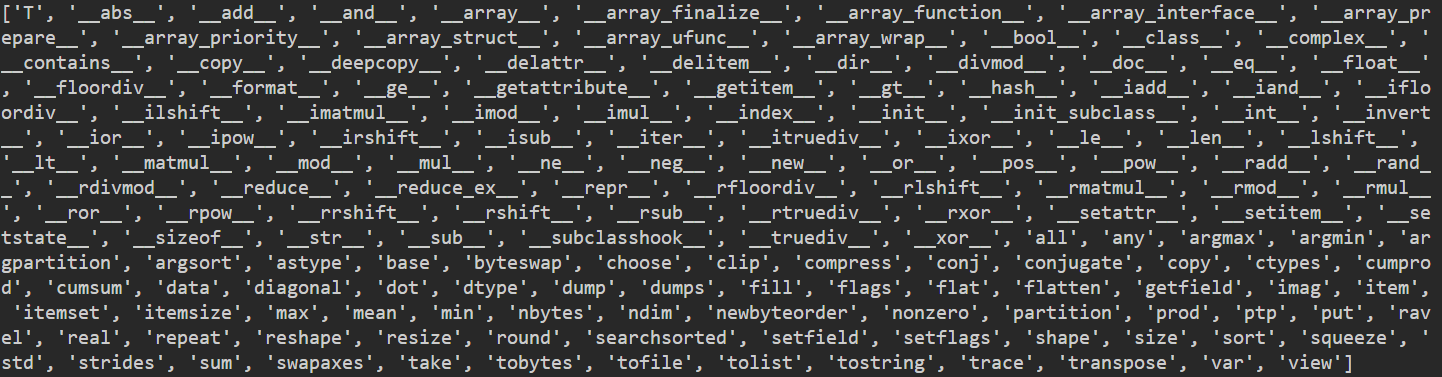
\includegraphics[width=10cm]{../figures/dir_ndarray}
  \end{center}
  Los métodos que empiezan y acaban con un doble  ``\_'' se llaman
  ``dunder'' (double underscore)  methods y son para uso interno del módulo.
  \end{itemize}
\end{frame}
  
\end{document}
